\title{Implementation of a Kalman Filter}
\author{Joseph Galante}
\documentclass{article}
\usepackage{graphicx}%needed for images
\usepackage{amsmath}%needed for bmatrix and operatorname
\begin{document}

\maketitle

\begin{center}
\Huge 
DRAFT
\normalsize
\end{center}
\vspace{4cm}

Disclaimer

This document is intended to allow a motivated student to understand the basics about how control strategies can be applied for depth control of an AUV.  This document is \emph{not} intended to be a suitable replacement for a classical course in control theory.  Without a thorough understanding of the underlying mathematics and concepts that are glossed over or skipped entirely in this paper, it can be dangerous for a novice to implement these strategies.  When in doubt, seek consultation or supervision from someone experienced.

\newpage

This document works through the implementation of a Kalman filter for the simple problem of determining the position of a box falling under the influence of gravity.  While the problem is relatively simple, the Kalman filter is an extremely powerful tool and can be applied to other far more complicated problems in a similar manner.  Section \ref{sec:probStatement} discusses the problem at hand and provides motivation for when a Kalman filter might be useful.  In Section \ref{sec:mathModel} the falling box problem is modeled mathematically.  The TODO STUFF GOES HERE


\section{Problem Statement}
\label{sec:probStatement}

\begin{figure}[h]
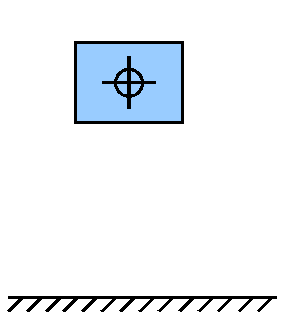
\includegraphics[scale=0.25]{boxPicture.png}
\centering
\caption{The problem: find the position of the box as it falls.}
\label{fig:boxPic}
\end{figure}

Consider a box that initially starts in midair and falls under the influence of gravity as shown in Figure \ref{fig:boxPic}.  This document examines the problem of determining the position of the box while it falls.  This might seem like a simple problem.  Perhaps you have seen in a basic physics or calculus course that the position of a box falling with constant acceleration can be derived by simple integration:

\begin{align}
\label{eq:naiveDynamics}
\ddot{x}(t) &= -g\nonumber\\
\dot{x}(t) 	& =\int_0^t\!\ddot{x}(\tau)d\tau 	= -gt+\dot{x}(0)\nonumber\\
x(t) 		&= \int_0^t\!\dot{x}(\tau)d\tau 	= -\frac{g}{2}t^2+\dot{x}(0)t+x(0)
\end{align}

Now the position of the box as a function of time can be solved if the exact initial position $x(0)$, the exact initial velocity $\dot{x}(0)$, gravitational constant $g$, and mass $m$ are known.  We certainly have a very good idea of the value of the gravitational constant $g$, but our knowledge of mass $m$ may not be perfect.  It is also likely that the initial conditions $x(0)$ and $\dot{x}(0)$ are only known to a certain degree of accuracy.  The dynamical model $\ddot{x}(t)=\frac{-g}{m}$ does not include drag which may be significant (especially if the box's velocity grows large).  The dynamical model also neglects random forces acting on the box, such as winds and thermal drafts.  It is clear that basic techniques from calculus and physics will not be of much use in determining the box's position if we consider complicated dynamical models, uncertainty in parameters, uncertainty in initial conditions, and random forces.  

If using a mathematical model isn't straightforward, perhaps the position of the box as it falls can be directly measured.  Assume that we can place an altimeter in the box that can report a measurement $y(t)$ of the position of the box $x(t)$ over time.  It would be wonderful if the measurement was exactly equal to the what we want to measure: $y(t)=x(t)$.  Unfortunately, in the real world it is often the case that a sensor has random noise $n(t)$ that corrupts the measurement in some way.  Sometimes sensors can be purchased that have noise that is so small it can be considered negligible; but these often come at high cost and may have undesireable weight, an incompatible form factor, or simply may not be available.  For most measurement systems, the practicing engineer is usually stuck with noisey measurements.  In the case of the falling box the altimeter measurements take the form $y(t)=x(t)+n(t)$. 

The Kalman filter is designed to optimally handle problems with any of the above situations.  Unfortunately, the full derivation of the Kalman filter is so complicated that it typically takes an entire graudate level course to thoroughly understand.  This document will attempt to explain how Kalman filters work by applying one to the falling box problem, but \emph{many} details will be omitted for brevity.  


\section{Mathematical Model}
\label{sec:mathModel}

The first step in analyzing any control or estimation problem is to construct a mathematical model of the situation.  In this problem we're looking at the motion of a box under the influence of several forces, so our mathematical model will come from the system dynamics.  A free body diagram, shown in Figure \ref{fig:boxFreeBodyDiagram}, is a useful tool to assist in writing the dynamic equations.

\begin{figure}[h]
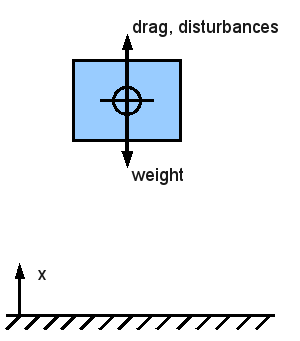
\includegraphics[scale=0.25]{boxFreeBodyDiagram.png}
\centering
\caption{Free body diagram of the box.  The weight of the box pulls it downwards.  Drag and disturbance forces have been drawn to act in the direction opposite of the weight. }
\label{fig:boxFreeBodyDiagram}
\end{figure}

As shown in Figure \ref{fig:boxFreeBodyDiagram}, we can model all the forces acting on the box.  For simplicity, we assume that the box acts like a particle with forces acting on it.\footnote{The problem would be more difficult if we treated the box like a rigid body with forces that aren't lined up with the box's center of gravity}  The following forces act on the box:
\begin{itemize}
\item weight $=mg$ which always acts downwards
\item drag $=c\dot{x}(t)$ with $c>0$ which is drawn so that the drag force is always opposite the direction of motion
\item disturbances $=d(t)$ which will be discussed in greater detail later 
\end{itemize}
We can now use Newton's Second Law to write the dynamic equation directly:

\begin{align}
\label{eq:dynamics}
m\ddot{x}(t) &= \sum F \nonumber \\
m\ddot{x}(t) &= -mg-c\dot{x}(t)+d(t)\nonumber\\
\ddot{x}(t) &= -g-\frac{c}{m}\dot{x}(t)-\frac{1}{m}d(t)
\end{align}

Control/Estimation people like to rearrange this equation into state space form.  Notice how Equation \ref{eq:naiveDynamics} is separable is is hence very easy to integrate (twice) to solve for $x(t)$.  Equation \ref{eq:dynamics} is more complicated.  While it can be solved for $x(t)$, this equation and others that are vastly more complicated can easily be solved by putting them in matrix form.  If we let $x_1(t)=x(t)$, $x_2(t)=\dot{x}(t)=\dot{x}_1(t)$, and $\pmb{x}(t)=\begin{bmatrix} x_1(t) \\ x_2(t) \end{bmatrix}$, then the state space form is:

\begin{equation}
\dot{\pmb{x}}(t) = \frac{d}{dt}\begin{bmatrix}x_1(t)\\x_2(t)\end{bmatrix}=\begin{bmatrix} 0 & 1\\ 0 & \frac{c}{m}\end{bmatrix} \begin{bmatrix}x_1(t) \\ x_2(t)\end{bmatrix}+\begin{bmatrix}0\\\frac{1}{m}\end{bmatrix}(-mg+d(t)) = A\pmb{x}(t)+B(-mg+d(t))
\end{equation}

\end{document}

